\chapter{Concepts and Architecture}

%\section{Prerequisite}


\section{Contracts}
First and foremost of the whole connectivity, protocol and bundling, the business contracts between the nodes has to be declared. Throughout the whole process of the these contracts and relationships between each participant got questioned and modified, since this is the most important aspect or basic building block for the whole thesis. 

\subsection{Client-ISP Contract}
In the first version of the FBP there are only two participants: Client and ISP. Before connecting, a contract between these two parties has to be closed. In this version it consists of the public key, private key, public key of the opponent and the feed ids of the ISP and Client feed. The public keys act as the name of each client or isp, the private keys are obviously used to write to the feed. The feed IDs act as identifier for in which feed has to be written or from which feed has to be read. \\\\
\begin{tabular}{llll} \toprule
    Client-Contract&value&ISP-contract&value\\ \midrule
    actual public key:& cli001 &  actual public key: &isp001  \\ 
    actual private key:& ****** & actual private key:& ****** \\
    actual feed ID:& cli001\_isp001 &actual feed ID:&isp001\_cli001 \\ 
    ISP public key&isp001&Client public key:&cli001\\
    ISP feed ID&isp001\_cli001&Client feed ID:&cli001\_isp001\\\bottomrule
\end{tabular}
\subsection{ISP-Server Contract}
Same as in the Client-ISP Contract.\\\\
\begin{tabular}{llllll} \toprule
    ISP-contract&value&Server-Contract&value\\ \midrule
    actual public key:& isp001 &  actual public key: &ser001   \\ 
    actual private key:& ****** & actual private key:& ******  \\
    actual feed ID:& isp001\_ser001 &actual feed ID:&ser001\_isp001\\ 
    Server public key:&ser001&ISP public key:&isp001\\
    Server feed ID:&ser001\_isp001&ISP feed ID:&isp001\_ser001\\\bottomrule
\end{tabular}
\\\\
Clearly seen, that client and server are 'connected' over isp001 - initial idea was a peer to peer isp network where the ISP-Company distributes the feeds and packages in a defined way - so actually isp could stand for swisscom and the number 001 the actual connectivity provider stations which means cli001 has a contract with isp342 and server has a contract with isp903. And swisscom has internal routing to pass information from isp342 to isp903.
\\
Result:

\begin{figure}
    \centering
    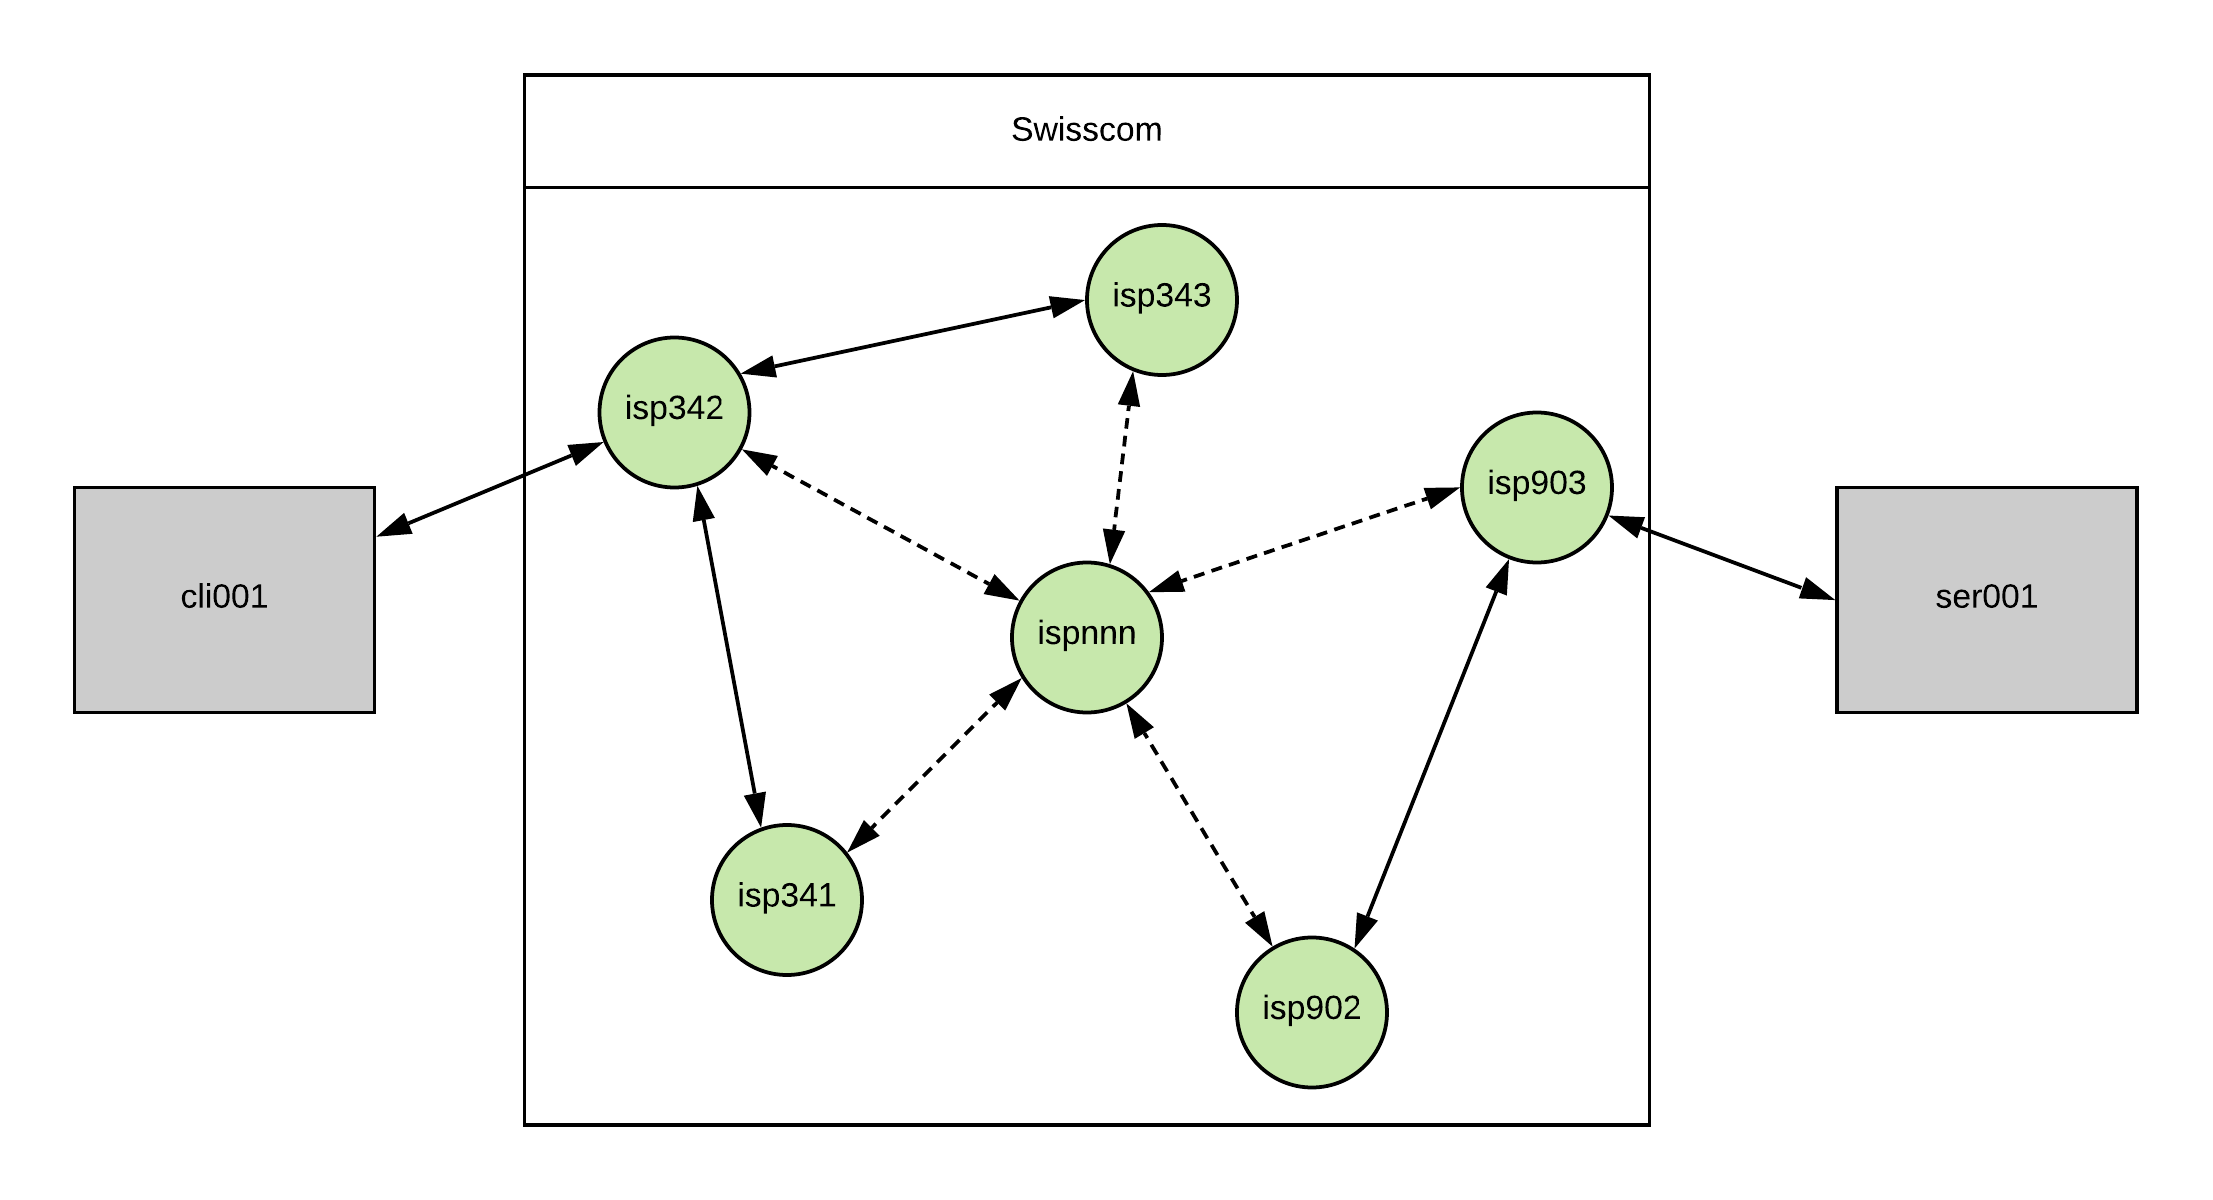
\includegraphics[width=0.9\textwidth]{p2p_contracts}
    \caption{A simplified contract network.}
    \label{fig:contract_network}
\end{figure}



Since now a contract is established, the client should hold information for the ISP and vice versa. This leads to the Feeds.

\pagebreak

\section{Feeds}
Feeds are append only logs/files. Which means there can only be written to or read from. There is no option to delete entries except by deleting the whole file. So a feed acts as database for all the requests made or information given in the context of the connection between client and isp.\\
\textit{more detailed information about schema of feed, hashchain, sequence and content}\\
\textit{also give context to keys - cryptography - signing}\\
\textit{role of the feeds in fbp and introducing the idea of feed pairs.}
Given in the contract these feed IDs are already defined and each node knows where to store or write its own information and read the peers information.
Result:

\begin{figure}
    \centering
    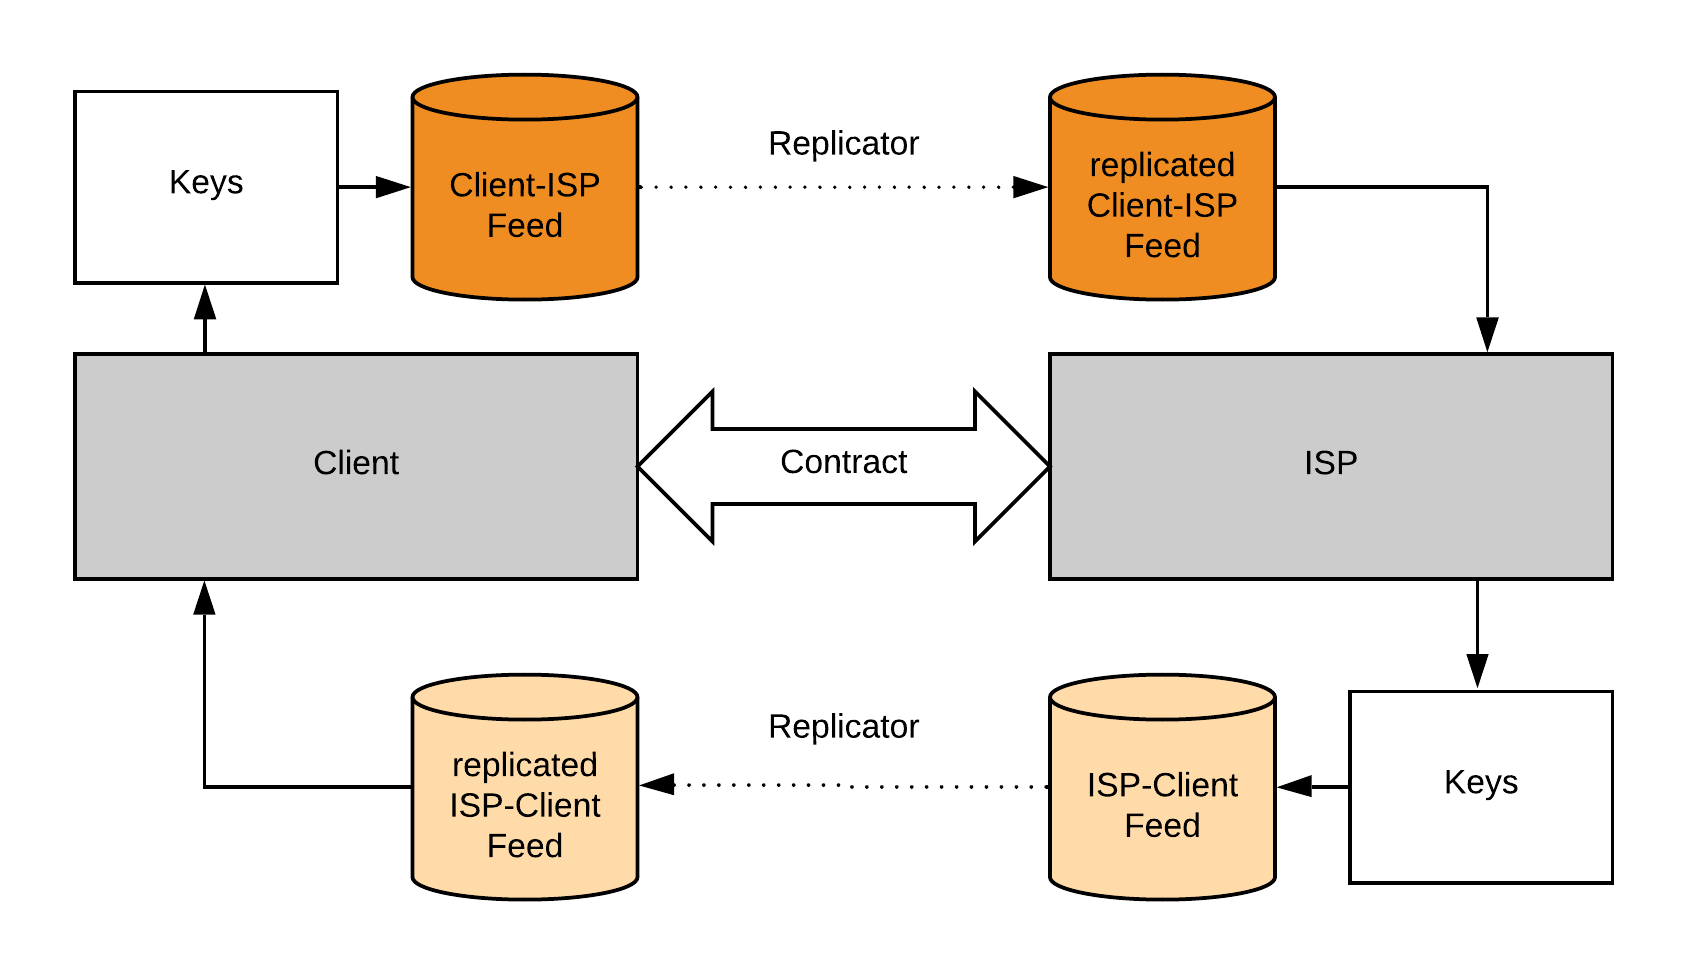
\includegraphics[width=0.9\textwidth]{fbp_v0_1_Schema}
    \caption{Full contract between client and ISP with feeds.}
    \label{fig:contract_cli_isp}
\end{figure}

Having this setup the next step is to have a possibility to communicate, so the client can request information from the isps real database

\pagebreak
\section{Remote Procedure Call}
General explanaiton of RPC.

\subsection{Send Request}
Format of request and api of method
\subsection{Read Request}
Format of request and api of method
\subsection{Send Result}
Format of request and api of method
\subsection{Read Result}
Format of request and api of method

Resulting schema of the API and descriptions given above:

\begin{figure}
    \centering
    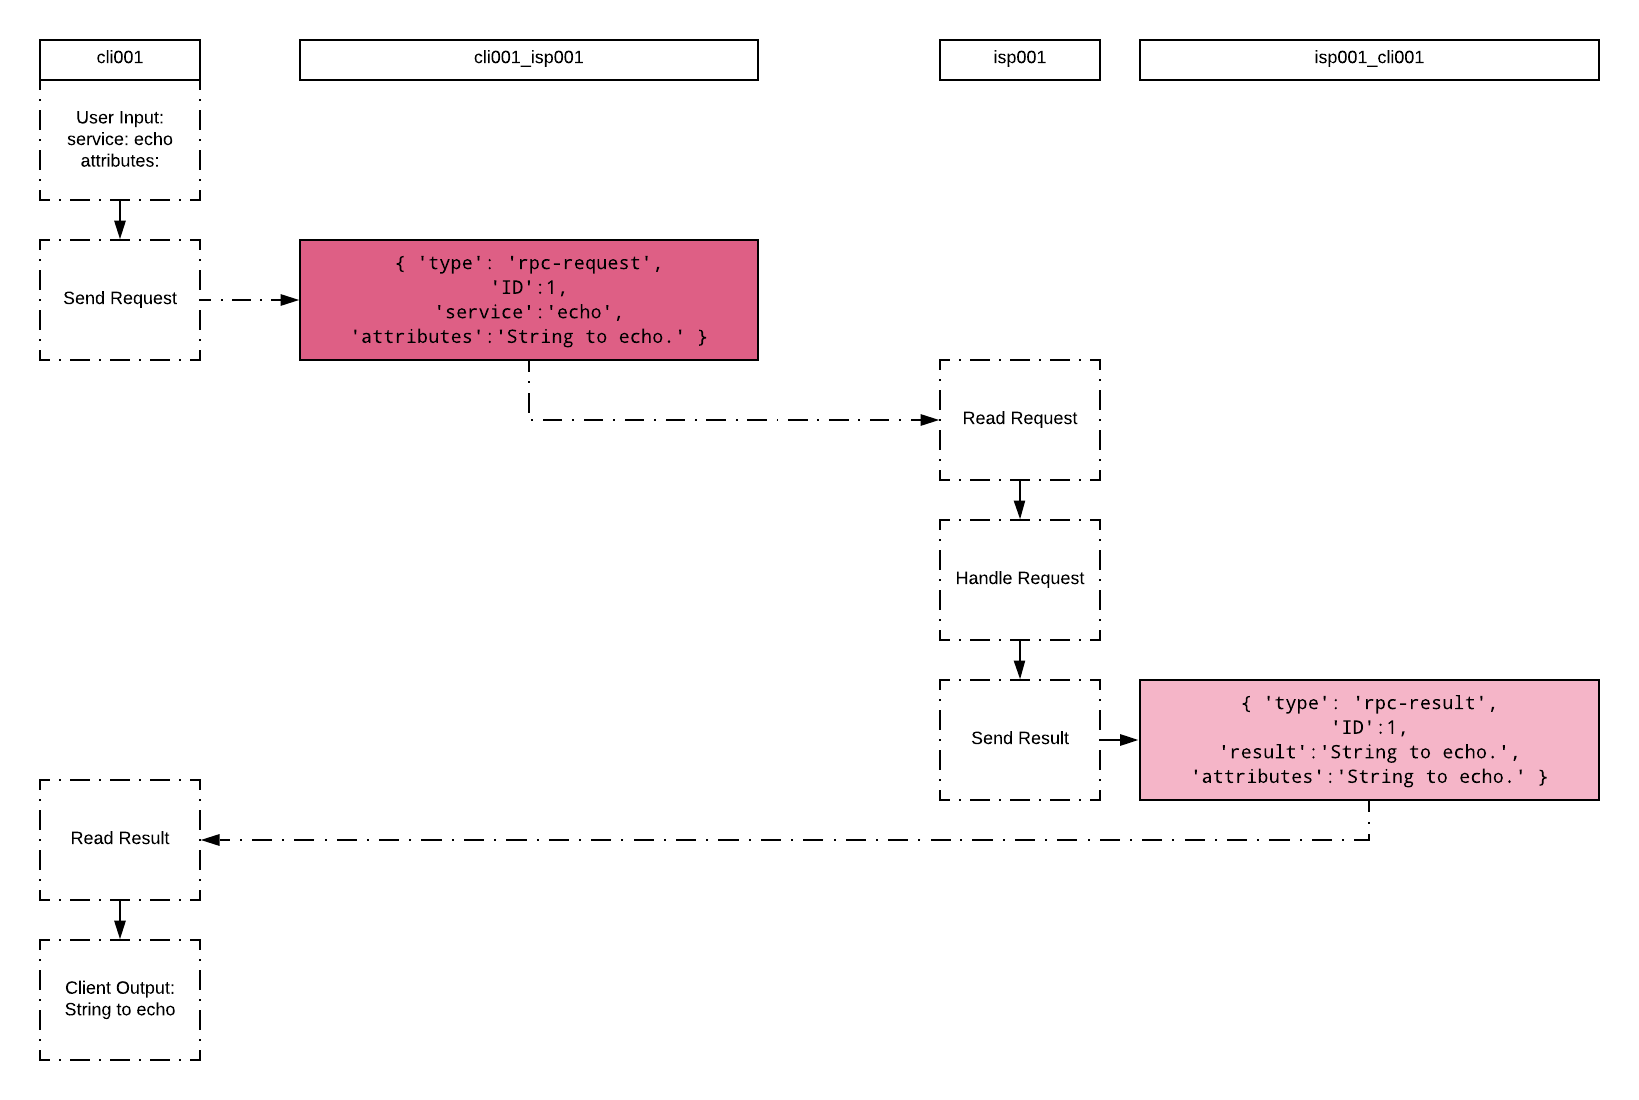
\includegraphics[width=0.9\textwidth]{rpc}
    \caption{A Remote Procedure Call by cli001 to isp001.}
    \label{fig:contract_cli_isp}
\end{figure}


Picture description: -> will be splited into above sections

Seen in the picture above, client cli001 makes a request of the echo service with the attribute: String to echo. This is passed to the send\_request function which assigns an unique ID for this request, resulting from the already given ids in the feed pair. Also merges type, id, service, and attributes into a request (a defined datastructure), writes appends this as a new log entry to the feed and saves the ID for keeping track of open requests. isp001 now detects a change on the feed cli001\_isp001 and invokes the read\_request method which takes the request appart and evaluates the service. Now the request gets handled and the wanted value returned. After that send result is invoked. It is similar to the send request, difference is the type and the result is also appended to the result datastructure. Now again, writing a new log entry to the feed with the given content. cli001 is notified that the isp001\_cli001 feed is changed. so read result is invoked and the result gets either to the program, where it was requested or printed to the client.

%\section{v0.2}
%The next step was to include servers with services. Also here the Prerequisite and contract situation changed.
\section{Introducing and Detrucing}
\subsection{Introducing}
General Idea - 
onboarding to a server. Instead of following server - introduce to server. differs from pub sub pattern in the way that the server has the choice to accept or decline a client. in either way accept or decline an answer is provided to the client.

procedure - cli001 sends rpc request with service:introduce, attribute:ser001 to isp001.
isp001 now makes rpc request with information about client and the fact, taht it wants to introduce itself to ser001 since they have a contract. 
if ser001 accepts introduce and creates from information sub feed - feed with communication direct between client and server.
result is contract information for client given by server: feed ID etc.
else ser001 declines, so result is no contract.
isp001 gets the result and passes this result to the initial rpc request from the client. client now gets result - also builds subfeed according to contract and connection is established. now if client wants to use a service from server it only writes the request in the corresponding feed and procedure is the same as described in RPC Section.
\\
important addition, only client can introduce, so only client can ask server for a contract. server has no information about any cient in the network at initial state.
\subsection{Detrucing}
Detrucing as a newly invented word by me, since normally after you introduced yourself to a person there is no way to make this unhappened. it acts the same for unfollow in a pub sub domain. But in contrary to the introduce both parts of the contract can detruce. \\
precisely either client or server can send rpc request to isp service detruce which gets propagated to opponent and results in terminating the whole contract. -> deleting keys and feeds.
\\
Important addition: after detruce client can again introduce to server.

Resulting picture:
\begin{figure}
    \centering
    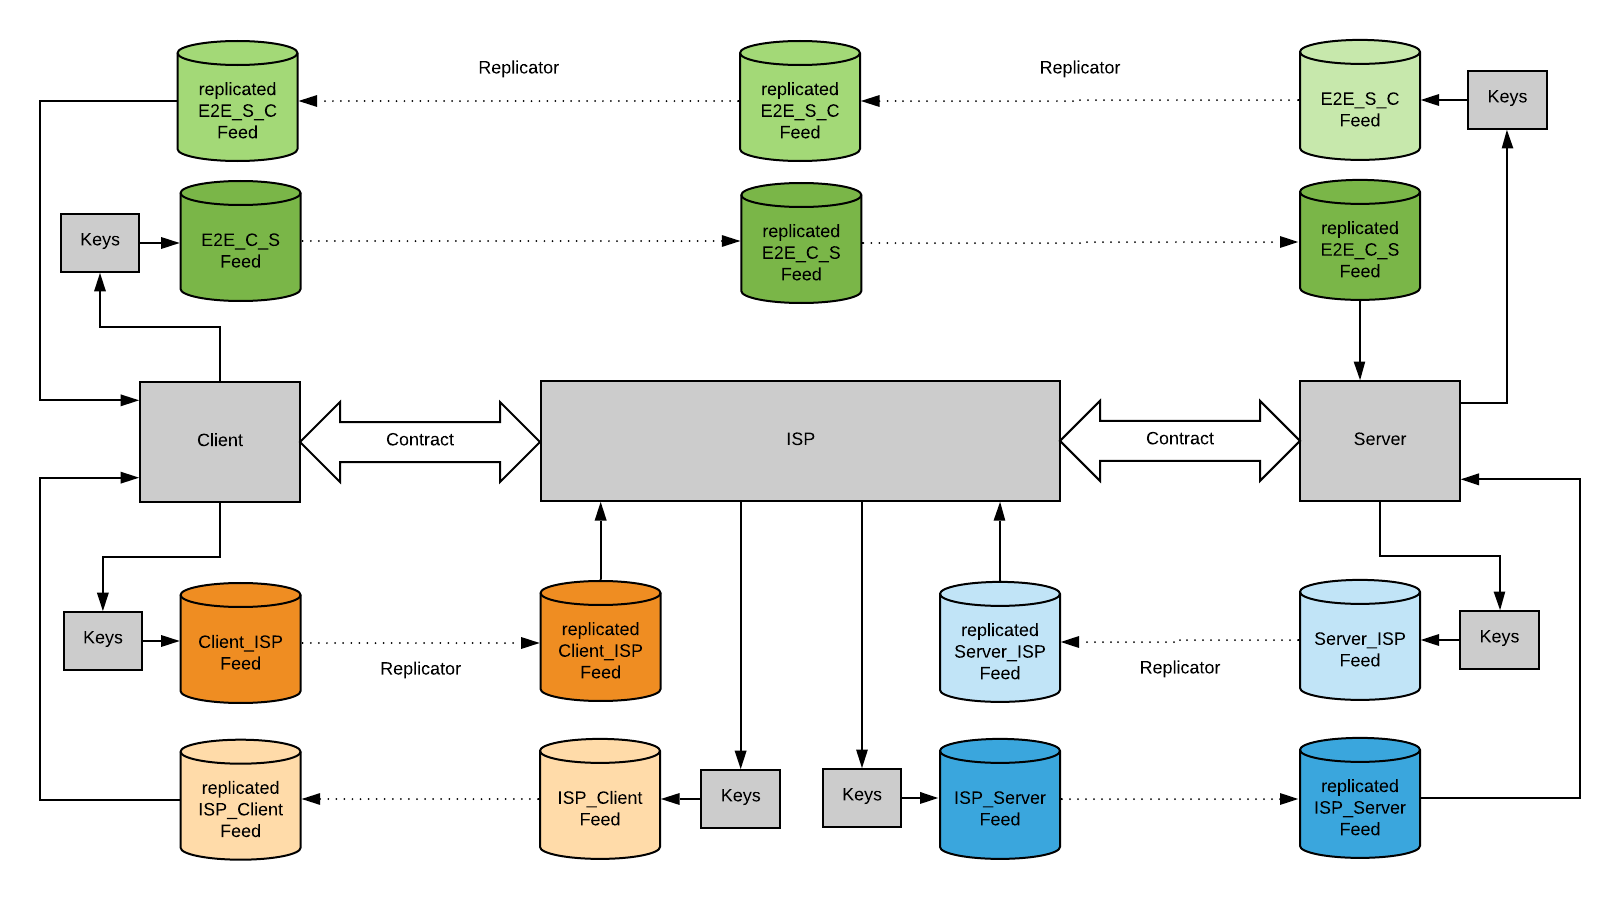
\includegraphics[width=0.9\textwidth]{intro_detru}
    \caption{State after accepted introduce from cli001 to ser001}
    \label{fig:contract_cli_isp}
\end{figure}

\pagebreak
\section{Replication}
locally in testing environement this above works. for real world application there needs to be a replication mechanism which propagates feeds to destination.

feed replication works at each write to the feed, to the  defined location.\\

API\\

could be erweitert to many destinations with an easy effort

resulting picture:
\begin{figure}
    \centering
    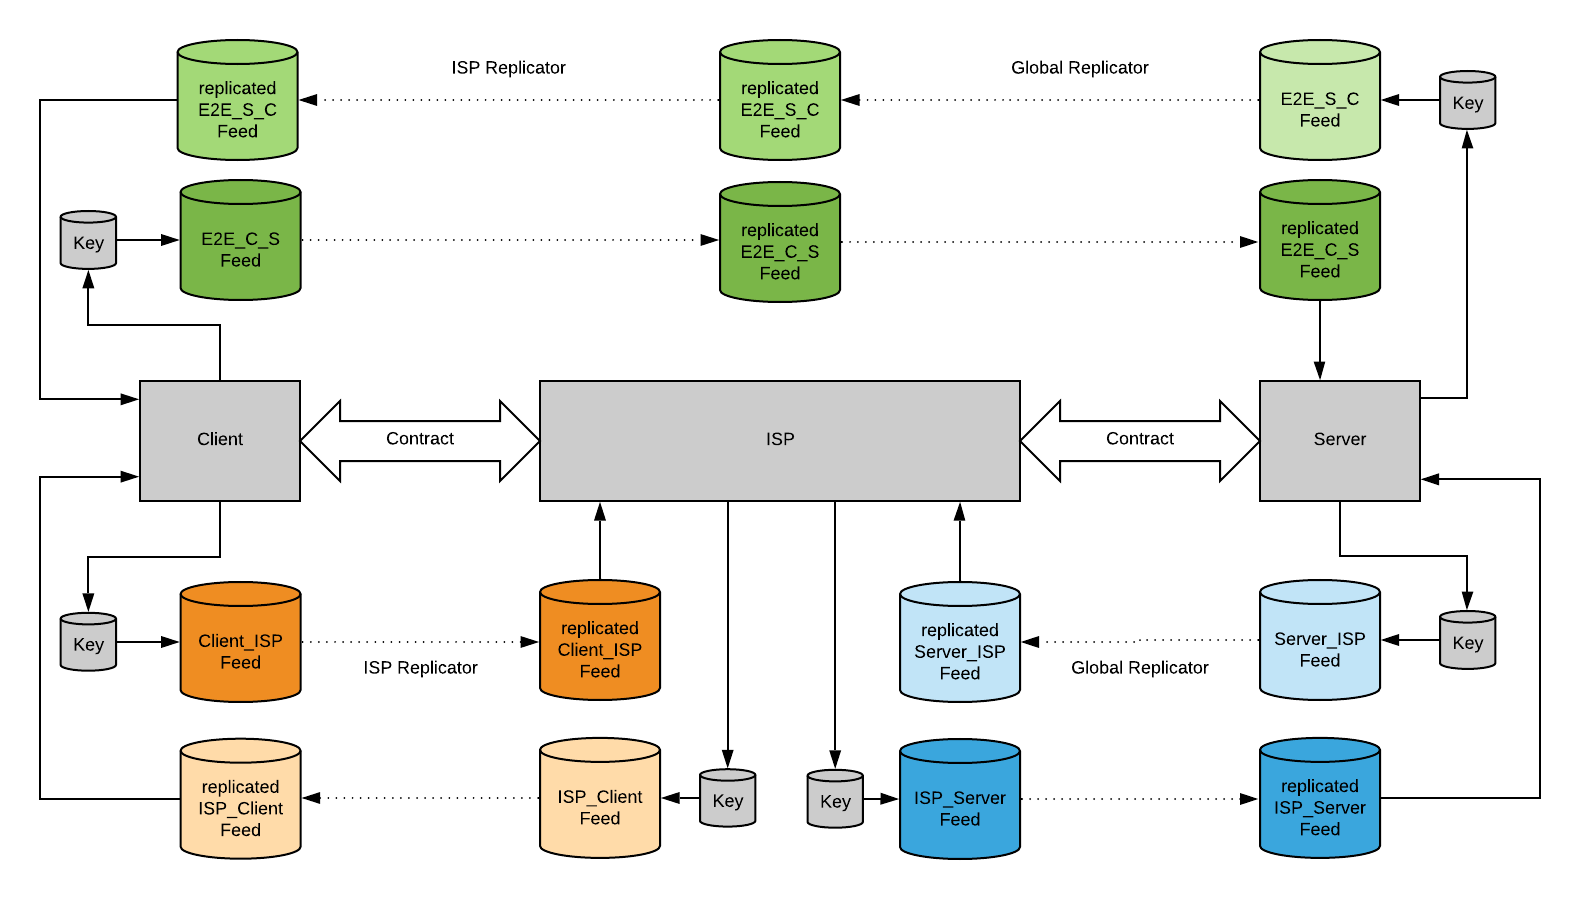
\includegraphics[width=0.9\textwidth]{replicator}
    \caption{Replicated Feeds}
    \label{fig:replication}
\end{figure}

seen that e2e feed pair between client and server now are replicated over isp node.\\ 
now bundling can be provided.

%\section{0.4}
%added indirect communication from client to server over ISP\\
\section{Bundling}
taking again a look at the real world problem the isp has arbitrary many clients and many of them want to cumminicate with the same server. Idea: bundling all e2e feeds to same server into isp-server feed.
-> load on wire problem

\subsection{Adapted Introducing and Detrucing}
introducing to server same - after server accept server generates both feeds request and result feed - sends contract to isp and isp generates result feed and replicates to cli - finally client generates request feed and replicates to isp.


\subsection{Multiplexing and Demultiplexing}
requests from client same way to isp. but isp does not replicate feed anymore. it takes whole log entry, signed by client and mulutiplexes into a new log entry with a mux type content and signs this - mutliplexing. at server, server takes this mux type and extracts whole request feed entry and appends bytes to request feed from client - demultiplexing. handles request and writes result to result feed. from there the whole entry gets again multiplexed in the ispser feed. at isp isp demux entry and also appends bytewise to result feed. replicates to cli and cli can use result.

Resulting Schema:

\begin{figure}
    \centering
    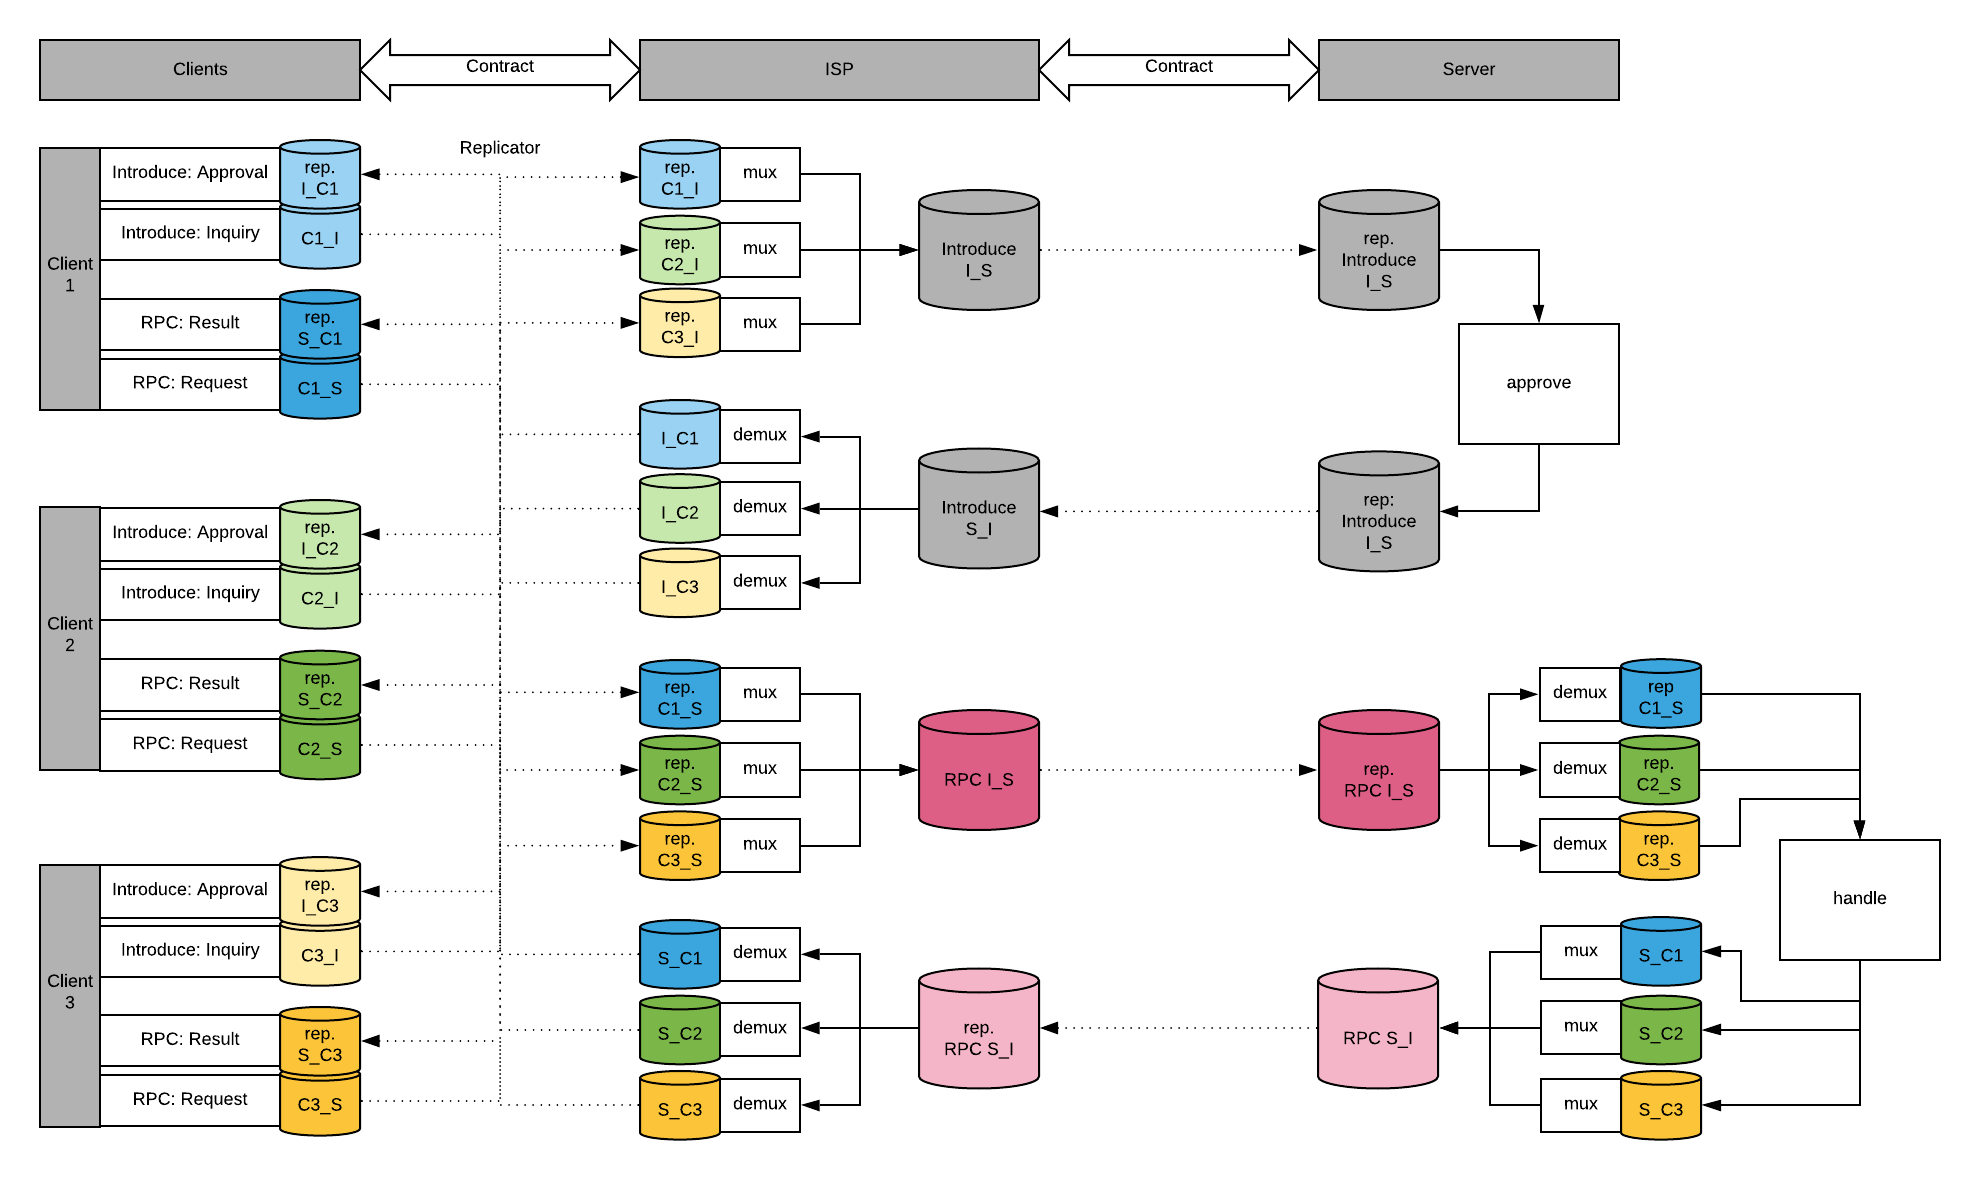
\includegraphics[width=0.9\textwidth]{mux_schema}
    \caption{multiplexing}
    \label{fig:mux}
\end{figure}

\section{Outlook}
\subsection{P2P ISP Nodes}
\subsection{Contract between ISPs}